\chapter{The search for diphoton resonances}
\label{chapter:diphoton}

In this chapter the search for resonant BSM production of photons pairs is presented.
First the analysis approach and event selections optimization are described, then
the statistical analysis and finally the results.

The analysis has been optimized for searches performed on data collected from proton-proton
collisions at a center of mass energy of 13 TeV and the results are obtained from the analysis
of \lumisix of p-p collisions collected by the CMS experiment during 2016. 

% The photon identification optimization has been performed with
% data collected during 2015 corresponding to an integrated luminosity of \lumififBon.

\section{Analysis approach}
The analysis is optimized to select a pure sample of diphoton events to fit the resulting
invariant mass spectrum with a model describing both the background and the hypothetical signal
coming from BSM resonances. Given the pure signature of the diphoton event the main background
is the standard model production (see Section~\ref{sec:sm_dipho_prod}) with a marginal contribution
from events in which one or both photons are mis-identified hadronic jets. The purity of the sample
is found to be more than $90\%$ but no attempt is made to separate the various background contribution
and the overall background shape is model with a parametric function.

Both the signal model shape and normalization from simulation are corrected for detector effects using
data-driven techniques which involves \Zee events. The general assumption is that the CMS ECAL
responses to electrons and photons are equivalent. 

\section{Data samples}
\label{sec:diphotons_data_samples}
The search is perform in data collected by the CMS experiment during the year 2016. The total
integrated luminosity is \lumisix. Data are reconstructed with a detector calibration optimized
for the 2016 p-p collision data-taking period using data collected in 2015 with the method described in
Section~\ref{sec:calib_2015}. The calibration described in Section~\ref{sec:calib_2016}
provides an improved ECAL energy scale stability which in turn leads through a better resolution
to a higher sensitivity of the analysis to narrow resonances and also to an improved stability
of some the variables included in the photon identification. However the technique was developed
well after the end of the data-taking and given the limited number of analysis that could potentially
profit from the improved performance a reconstruction with the new calibration was delayed and will become
available by the end of 2017. The response variations observed in 2016 and described in details in Section~\ref{sec:calib_2016}
are corrected with another method described in Section~\ref{sec:dipho_energy},
which does not correct for the PN diode blocks as the improved technique but only for global scale variations, separately
for the ECAL barrel and endcaps.

The events were recorded with a trigger designed to select events containing a pair of
energetic photons with $E_T > 60$ GeV. The energy of each photon candidate is computed as
the sum of the energy measured by ECAL and HCAL and trigger selections require
the energy measured in HCAL to be less than $10(15)\%$ of that measured by ECAL for candidates
in the calorimeter barrel(endcap) region.
The trigger is found to be fully efficient for photons with $\pt > 75$ GeV and so an offline
selection is applied to select these events.

Together with the main analysis trigger another one is used to select electrons from \Zee decays.
The \Zee is the primary control sample of the analysis and events compatible with this process
are recorded with a single electron trigger that selects events with at least one electron of
$\pt > 27$ GeV and $|\eta| < 2.5$. Tight isolation and identification criteria are applied at trigger
level to maintain a rate compatible with the DAQ capabilities.
\Zee events are used to measure the final photon selection efficiency so the single electron trigger
is preferred over a double electron one, since in this way an unbiased set of electrons can be
constructed from those coming from \Zee decays that did not triggered the event acquisition.

\clearpage
\section{Monte Carlo simulated samples}
The Monte Carlo simulation of the CMS detector and 13 TeV p-p collisions is used. The simulation
takes into account both the pileup generated by concurrent interactions and the presence of
signals in the detector coming from collisions in other bunch crossing. Events in the simulated samples
are re-weighted to match the pileup energy density distribution measured in data.

\subsection{Resonant signal simulation}
\RS gravitons are chosen as a reference for the spin-2 resonance search. SM-like Higgs bosons of high mass and
fixed widths are used for the spin-0 case.
A set of simulation samples is used to model the detector response to resonant production of two photons.
Such samples are generated with PYTHIA8~\cite{pythia8} in the mass range $500 < \mgg < 7000$ GeV in steps of 250 GeV for
masses below 4 TeV and 500 GeV above it. An additional set of samples without simulation of the detector
response are used to model the signal spectrum and the acceptance of the kinematic selections.
Three relative width hypothesis $\Gamma/\mgg$ are taken as benchmarks: $0.014\%$, $1.4\%$ and $5.6\%$ which,
in the case of \RS gravitons, correspond to a $k/M_{Pl}$ of $0.01$, $0.1$, $0.2$ respectively.
The trigger reconstruction and selections are simulated in these samples and the double photon trigger
used in the analysis is found to be fully efficient for signal events at all masses (Figure~\ref{fig:trig_eff_sig}).

\begin{figure}[h!]
  \centering
  \includegraphics[width = .45\textwidth]{figures/diphotons/eff_dipho60_EBEB_vs_mass.pdf}
  \includegraphics[width = .45\textwidth]{figures/diphotons/eff_dipho60_EBEE_vs_mass.pdf}
  \caption{HLT trigger selection efficiency as a function of the simulated resonance mass. Only events where the two photons are
    in the detector acceptance are considered. The left (right) plot refers to events in the EBEB (EBEE)
    category (see Section~\ref{sec:event_cats})}
  \label{fig:trig_eff_sig}
\end{figure}

\subsection{Standard model diphoton production simulation}
Even though the shape and yield of SM non-resonant diphoton production are measured with fit to the data,
simulated samples of the background processes are used for analysis optimization. A set of QCD induced
$\gamma+jet$ events generated with PYTHIA8 is used to optimize the photon identification selections.
The events are produced in several invariant mass bins in order to have a significant amount of photons and
jets over the whole $p_T$ spectrum.

\subsection{Drell-Yan production of electron-positron pairs}
Finally a set of Drell-Yan events ($Z \to e^{+}e^{-}$) is generated with aMC@NLO and is
used to derive data to simulation scale factors for the selections efficiency. This sample is generated
as a pure, unphysical, set of Z boson decays, neglecting the interference with the photon.

\clearpage
\section{Events selection}
\label{sec:dipho_selection}
Two measurement are needed to build the invariant mass of the diphoton system: the energy of the
photons and the position of the primary interaction. The former is performed with the ECAL as described in
Section~\ref{sec:ecal_reco} while the latter is reconstructed with tracks produced in the hard scattering against which
the diphoton system recoils. Additional information from the tracker and the HCAL are used to discriminate
genuine photon candidates from QCD jets.
In the following paragraphs the vertex and photon identification algorithms are presented.

\subsection{Vertex identification}
The standard CMS reconstruction identifies the primary interaction vertex (PV) as the one 
that as the largest $\Sigma p_T^2$ within each bunch crossing (where the sum runs over all the charged particles
coming from the vertex). The method is not fully efficient for diphoton events since the two neutral
particles carry a significant amount of the transverse energy.
A dedicated boosted decision tree regression has been trained in the context of the search for the
Higgs boson decaying into two photons~\cite{Khachatryan:2014ira}. Inputs to the regression are the $\Sigma p_T^2$ and
other quantities related to the $p_T$ balance between the diphoton system and the charged particles.
Using this method the interaction vertex is correctly assigned for about $90\%$ of the signal events.

\subsection{Kinematic selections and event categorization}
\label{sec:event_cats}
Photons candidates are reconstructed from energy deposit in the ECAL with no associated track.
A set of kinematic selection is applied to avoid detector inefficiencies and shaping of the mass
spectrum due to trigger level selections:
\begin{itemize}
\item The transverse momentum of each candidate greater than $75$ GeV.
\item The absolute value of the pseudorapidity of the supercluster (\absScEta) of both
candidates is required to be below $\absScEta < 2.5$ and not between $1.4442 < \absScEta < 1.566$,
due to the geometric acceptance of the ECAL. Photons in the region $2.5 < |\eta| < 3.0$ are still detected by the ECAL
but the absence of tracker coverage limits the discrimination between photons and jets, furthermore signal photons
are more likely to be produced in the central region of the detector.
\item To avoid a distortion of the background shape due to the transverse momentum
  cut, the minimum invariant mass of the diphoton pair has to be $230$ GeV, when
both photons are detected in the ECAL barrel region (EB, $\absScEta < 1.4442$). If one photon candidate
is detected in the endcap region (EE, $\absScEta > 1.566$), the minimum invariant mass
has to be $330$ GeV.
\end{itemize}

If more then one pair of photons satisfies the kinematic selection ($1\%$ of all the events) the pair
with the highest scalar sum of transverse momentum $p_T^{\gamma\gamma}$ is chosen.

The events are split into two categories accordingly to the topology of the photon system in relation
to the ECAL segmentation:
\begin{itemize}
\item barrel-barrel (EBEB): both photons are detected in the ECAL barrel region $\absScEta < 1.4442$.
\item barrel-endcap (EBEE): one photon is detected in the ECAL barrel region $\absScEta < 1.4442$ the other
  in one of the endcaps $1.566 < \absScEta < 2.5$.
\end{itemize}

The EEEE category (both photons detected in the endcaps regions) is not considered for the analysis
since only few percent of the benchmark signal events fall in this category and conversely the SM
background is considerably higher than in the other categories.

\subsection{Photon identification}
Energetic neutral pions found in QCD jets has a signature similar to that of a photon since they decay into two collimated
photons. A dedicated set of selection is applied to each photon candidate in the analysis to select a pure
sample of diphoton events. These criteria were optimized for photons with high transverse
momentum and based on the following variables:

\begin{itemize}  
\item \chIso: the scalar sum of the transverse momenta of the particle flow charged hadron
candidates (see Section~\ref{sec:cms_pf}) , which are assigned to the chosen primary vertex. Only candidate
within a radius of $\DeltaR < 0.3$ from the photon in the $\eta$ - $\phi$ plane, which is
defined as:
\[
\DeltaR = \sqrt{(\eta_\gamma-\eta_{cand})^2 + (\phi_\gamma-\phi_{cand})^2}
  \]
are considered.

\item \phoIso: the scalar sum of the transverse energies of the particle flow photon candidates for which $\DeltaR < 0.3$.
  
\item \hoe: ratio of the energy measured in the HCAL and ECAL.

\item \sieie: the weighted spatial second order moment of the photon candidate in the
  $\eta$-direction, computed as:
  \[
    \sieie = \sqrt{ \frac 
      { \sum_{i \in 5\times5} \left( \eta_i - \bar \eta \right )^2 w_i
      } {\sum_{i \in 5\times5} w_i} }, ~~~~ 
    w_i = \max \left( 0, 4.7 + \log(E_i / E_{5\times5}) \right )
\]

% \item \rnine: the ratio between the energy of the 3x3 crystals around the most energetic crystal and the energy of the whole supercluster.

\item Conversion safe electron veto, to reject electrons.

\end{itemize}

Particle flow charged particles or photons sharing part of their energy with the photon candidates
are excluded from the \chIso and \phoIso sum. 

The selection value are reported in the following table:

\begin{table}[h!]
    \centering 
    \begin{tabular}{l|r|r|r|r}
        \hline
        photon category       & \chIso cut (\GeV) & $\phoIso^{corr}$ cut (\GeV)& \hoe cut & \sieie  cut \\
        \hline
        $\scEta<1.4442$ non-sat.  & 5                 & 2.75  &  $5 \times 10^{-2}$ & 0.0105 \\
        $\scEta<1.4442$ sat.      & 5                 & 2.75  &  $5 \times 10^{-2}$ & 0.0112 \\
        $\scEta>1.566$  non-sat.  & 5                 & 2.0  &  $5 \times 10^{-2}$ & 0.028 \\
        $\scEta>1.566$  sat.      & 5                 & 2.0  &  $5 \times 10^{-2}$ & 0.030 \\
		\multicolumn{5}{l}{conversion-safe electron veto applied for all categories} \\
		\hline
    \end{tabular}
    \caption{\label{tab:photon_id}
      Photon identification criteria used in the analysis. $\phoIso^{corr}$ is the corrected \phoIso value described
      at the end of this section.
    }
\end{table}

For very energetic photons the ECAL readout electronics can saturate. In such a case the shower shape variable
\sieie is distorted, hence a different selection value is set for this identification variable in case of saturation.

The thresholds of the identification variables were optimized to give an efficiency flat as a function
of the mass of the diphoton pair, the chosen working point correspond to an efficiency of $90(85)\%$ for
photons in the EB(EE).
The \phoIso distribution is found to depend on the event pile-up and the $p_T$ of the
photon candidate (Figure~\ref{fig:phoiso_qtiles}).
These dependencies leads to a variation of the selection efficiency with time and also
for different values of \mgg. In order to keep a flat efficiency an effective correction is used, its expression is:
\[
  \phoIso^{corr} = \phoIso - \kappa\cdot p_T - A \cdot \rho + \alpha
\]

where $p_T$ is the transverse momentum of the photon candidate, $\rho$ is the event pile-up energy density.
The values of $A$ and $\kappa$ are chosen such to keep the $90\%$ quantile of the distribution at a constant
value as a function of $\rho$ and $p_T$, while the $\alpha$ parameter is used to adjust the distribution such
that the bulk of the corrected isolation distribution for signal photons peaks at zero.

\begin{figure}[!h]
  \centering
  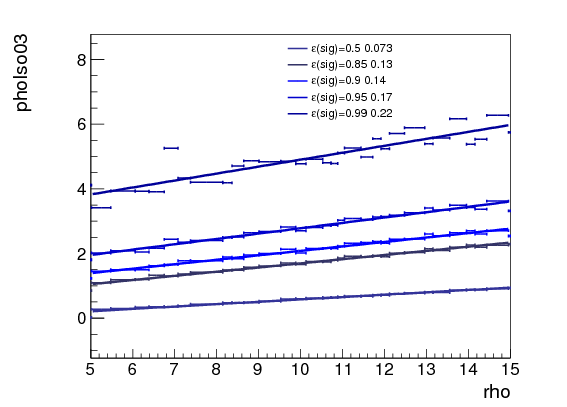
\includegraphics[width = .45\textwidth]{figures/diphotons/qtiles_phoIso03_outerEB.png}
  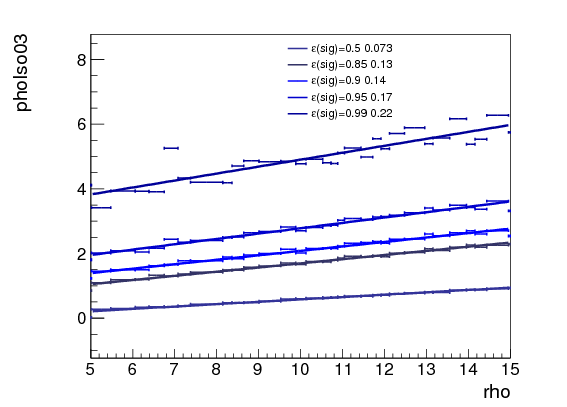
\includegraphics[width = .45\textwidth]{figures/diphotons/qtiles_phoIso03_outerEB.png}
  \caption{\phoIso quantile distribution as a function of the pile-up energy density for candidates in the EB  (left) and
    EE (right). The lines are fit to the points and are used to derive the correction described in the text.
  The slope at the 0.9 quantile is steeper than the one of the median, thus the need of the scale parameter $\alpha$}
  \label{fig:phoiso_qtiles}
\end{figure}

The values of the correction parameters are reported in Table~\ref{tab:pho_iso_corr}, $A$ is derived in five
bins of $|\eta|$ while two bins (barrel and endcaps) are sufficient for $\kappa$ and $\alpha$
to fully correct the $\rho$ and $\pt$ dependency of \phoIso.

\begin{table}[h!]
    \centering 
    \begin{tabular}{l|r|r|r}
        \hline
        region                & $\alpha$ (\GeV) & A     &  $\kappa$ ($1/\GeV)$ \\
        \hline                                          
        $\scEta<0.9$          & 0.99             & 0.15  &  $1.6  \times 10^{-3}$  \\
        $0.9<\scEta<1.4442$   & 0.99             & 0.13  &  $1.6  \times 10^{-3}$  \\
        $1.566<\scEta<2.0$    & 1.52             & 0.093 &  $0.75 \times 10^{-3}$  \\
        $2.0<\scEta<2.2$      & 1.52             & 0.15  &  $0.75 \times 10^{-3}$  \\
        $2.2<\scEta<2.5$      & 1.52             & 0.21  &  $0.75 \times 10^{-3}$  \\
        
		\hline
    \end{tabular}
    \caption{\label{tab:pho_iso_corr}
      Corrections factors for the \phoIso variable.
    }
\end{table}

% The reason behind the pile-up dependency is quite clear: neutral particles from pile-up cannot be filtered out
% by a particle vertex maching since no tracking infromation is available for neutral. A variation in the pile-up thus
% leads to a different average contribution of pile-up energy to the isolation cone around a candidate photon.

\subsection{Selection efficiency measurement}
\label{sec:dipho_eff}
The efficiency of the photon identification described in the previous chapter is measured in data
using the \Zee control sample. The measurement of the selection efficiency in data is then
compared to the one measured in the simulation and in case of discrepancy the signal normalization
derived from the simulation is corrected for the measured scale factor.

The efficiency is measured with a tag-and-probe technique exploiting the well known Z decay to electrons.
For this study the response of the ECAL and HCAL is assumed to be identical for electrons and photons.
The tag-and-probe method is used both for the data and simulation measurement, the \Zee control sample
in data is selected using events recorded with a single electron trigger (as described in Section~\ref{sec:diphotons_data_samples}).
Dielectron candidates
are further filtered with an invariant mass selection ($70 < \mee < 110$ GeV) centered around the Z mass peak,
the invariant mass window is applied also to the simulated events.

The method then requires one of the two electrons (the ``tag'') coming from the Z boson to pass a very tight selection
(this tight working point is developed by a dedicated group within CMS and provide high purity electrons
with an efficiency of $70\%$).
The second electron is required to pass a loose identification and is assumed to be unbiased
with respect the variables being studied (the ``probe''). The photon selection efficiency is studied using
this unbiased sample inverting the electron veto request.
The efficiency is studied as a function of the probe electron $p_T$.
%and the event pile-up energy density $\rho$.

The data  events are fitted
simultaneously for passing and failing probes with a signal plus background model.
The signal is modeled by the Z lineshape as obtained from a QCD NLO (POWHEG)
generator convolved with a Gaussian, while the background is modeled by an exponential function. As
the choice of the fit model is one of the dominating systematics, different models were
studied to assess it. A simple cut-and-count method is applied for the simulation sample
since the non resonant $pp \to \gamma^* \to e^+e^-$ events can be discarded with MC truth information and
are anyway not simulated in the sample used for this analysis.

The efficiency measurement is summarized in Figure~\ref{fig:tnp}: a good agreement between data and simulation is
observed across the whole probe electron $p_T$ spectrum and both for probes in the  ECAL barrel and endcaps, thus no scale factor
is applied to the predicted signal yield.

\begin{figure}
  \centering
  \includegraphics[width = .45\textwidth]{figures/diphotons/sf_vs_pt_EB.pdf}
  \includegraphics[width = .45\textwidth]{figures/diphotons/sf_vs_pt_EE.pdf}
  \caption{Efficiency measurement with \Zee events for electrons in the EB (left) and in the EE (right).
    The error bars on the data points
    account for the uncertainty originated from the choice of the fit model as described in the text.
    The bottom panels show the ratio between the efficiencies measured in data and simulation, the scale factor is
    compatible with unity within the uncertainties.}
  \label{fig:tnp}    
\end{figure}

% The analysis performed with \Zee events proves a good agreement between data and simulation up to 300 GeV of the electron
% $p_T$, at higher energies the efficiency is measured using 
% while the energy range explored by the main analysis extend to much higher energies. The effiency of the photon identification
% is measured  

\clearpage
\section{Photon energy scale and resolution corrections}
\label{sec:dipho_energy}
The detector response is simulated with fixed pile-up distribution, detector noise and transparency loss.
The pile-up distribution is re-weighted to match the one in data.
The detector noise and crystal transparency instead varies over the data-taking period and so a discrepancy
in the energy response of the ECAL may arise between data and simulation since in the latter no time evolution
of the detector conditions is simulated. The effect of this discrepancy translate in shift of the energy
scale in data with respect to the MC simulation (as described in Section~\ref{sec:calib_2016}),
furthermore any residual mis-calibration of the detector
is not simulated and thus the energy resolution in data is worse than in the MC simulation.
These two effects are corrected on one hand by
scaling the photon energy in data events
to correct the time dependent energy scale variations (see Section~\ref{sec:calib_2016})
and match the energy scale of the simulation and,
on the other hand, by smearing the energy in simulated events to match the resolution observed in data.

The time-dependent scale corrections and the smearing are derived with the \Zee control sample.
Again since the energy for both photons and electrons is primarily reconstructed from the ECAL, electrons
are used as a proxy of photons. The reader may notice that the energy reconstruction formula outlined in
Equation~\ref{eq:sc_energy} differs for electrons and photons in the supercluster energy correction term ($F_{e,\gamma}$).
Electrons used to derive the corrections described in this section are reconstructed the electron $F_e$ correction,
while both electrons used in the final data to simulation comparison and photons selected for the analysis
are reconstructed with the $F_{\gamma}$ correction factor.

The corrections are derived in two steps: in the first, the energy scale is corrected by
adjusting the scale in data to match the simulation prediction. The \Zee invariant mass peak is fitted with
a Breit-Wigner function convolved with a crystal ball (CB) function describing, respectively,
the theoretical signal line shape of the Z-boson and the detector response.
The parameters of the Breit-Wigner function for the Z boson are taken from the Particle
Data Group (PDG)~\cite{PDG}: $m_Z = 91.1876$ GeV and $\Gamma_Z = 2.4952$ GeV.
By fitting the distribution in data and MC simulation separately, the energy scale offset can be extracted.

Different systematic behaviors of the mean of the CB function ($\Delta_m$) as a function of time and the
pseudorapidity can be observed. As a result, run dependent energy corrections are
necessary to correct for the energy scale variations during data-taking. The energy scale
correction ($\Delta P$) is defined as the relative shift in mass between data and MC prediction:
\[
  \Delta P = \frac{\Delta m_{data} - \Delta m_{simulation}}{m_Z}
\]

After the $\Delta P$ correction is applied, a stable behavior of $\Delta m$ over time within
0.1 GeV is observed.

In the second step, the residual difference between the observed and predicted electron
energy is assessed by maximizing the likelihood between the smeared MC distribution and the data.

The smearing of the MC distribution is performed by multiplying \scE distribution by a
Gaussian distribution, centered at $1 + \Delta P$ and with resolution $\Delta C$.
The resolution $\Delta C$ denotes the additional constant term of the energy resolution which
is added to the MC prediction.

The additional constant term needed to match the energy resolution measured with data varies as a function
of \scEta, as the scale correction, but it also different between electrons that showers in the tracker volume
and those that don't.
The \rnine variable is used to discriminate between showering and non-showering electrons: this variables is used
instead of others since can also be applied to discriminate between converted and un-converted photons and
so is suitable to maintain the analogy between the analysis object (photons) and the control sample ones (electrons).
Thus maximum likelihood fit is performed in eight categories: four \scEta regions times two \rnine categories.

The comparison between the predicted and observed dielectron invariant mass spectrum around the Z boson peak,
for events passing the analysis selection (with inverted electron veto) and after all energy corrections have been applied
is reported if Figure~\ref{z_peaks}.

\begin{figure}[!h]
  \centering
  \includegraphics[width = .45\textwidth]{figures/diphotons/lowmass_EBEB.pdf}
  \includegraphics[width = .45\textwidth]{figures/diphotons/lowmass_EBEE.pdf}
  \caption{Comparison between predicted (shaded histogram) and observed (points) invariant mass distribution
    of electron pairs obtained after the application of energy scale and resolution corrections.
    The left figure refers to events where both electrons are detected in the ECAL barrel while the right one
    to events with one of the two electrons detected in the EB and the other in the EE.
    The simulation distribution is scaled to match the integrated luminosity of the data.
    The discrepancy in the right tail of both plots comes from the fact that the simulation do not include
  the non resonant Drell-Yan dielectron production and its interference with the Z boson.}
  \label{z_peaks}
\end{figure}  

Finally the linearity of the ECAL energy response is studied using Z bosons with high transverse momentum
decaying to electrons. This technique allows to test the linearity for transverse energies up to 150(100) GeV in
the EB(EE) region.
The linearity of the response is assessed by comparing the peak position of the
reconstructed Z mass measured in data and simulation as a function of $H_T = E_{T_1}^2 + E_{T_1}^2$, where
$E_{T_1,2}^2$ are the transverse energies of the two electrons.

For electrons detected in the barrel part of the detector, the corrected energy scale
is found to be stable within $0.5\%$. Electrons detected in the endcap region of the
detector are found to provide a stability of better than $0.8\%$.
A final $1\%$ uncertainty on the energy scale stability is assigned.
The smearing terms applied to the simulation in order to match the resolution observed in data are reported in
Table~\ref{tab:esmear_2016}. The additional constant term on the energy resolution varies from $0.96\%$ for
non-showering electrons in the barrel to $2.61\%$ for showering electrons in the forward region.

\begin{table}[!h]
 \begin{center}
   \begin{tabular}{|l|r|r|}
     \hline
     Category                   & $\Delta$C[\%] & $\Delta_{stat}$C[\%] \\ \hline
 $|\eta| < 1$ $R9 > 0.94$       & 0.96          & 0.07 \\
 $|\eta| < 1$ $R9 < 0.94$       & 1.03          & 0.11 \\
 $1 < |\eta| < 1.5$ $R9 > 0.94$ & 1.36          & 0.14 \\
 $1 < |\eta| < 1.5$ $R9 < 0.94$ & 1.82          & 0.05 \\
 $1.5 < |\eta| < 2$ $R9 > 0.94$ & 1.91          & 0.07 \\
 $1.5 < |\eta| < 2$ $R9 < 0.94$ & 2.20          & 0.13 \\
 $|\eta| > 2$ $R9 > 0.94$       & 2.53          & 0.13 \\
 $|\eta| > 2$ $R9 < 0.94$       & 2.61          & 0.10 \\
   \hline
   \end{tabular}
   \caption{Smearing values with uncertainty applied to the simulation in order to match the resolution measured in data.
     The values are extracted with the procedure described in the text and the uncertainties are of statistical nature
     and comes from results of the fit.}
    \label{tab:esmear_2016}
  \end{center}
\end{table}

\clearpage
\section{Statistical interpretation of the observed \mgg spectrum}
\label{sec:results}

This section presents the statistical technique used to interpret the analysis results.
The goal of the statistical analysis is to define a compatibility between the observed dataset
with the predicted standard model only and standard model background plus signal hypothesis.
Where no deviation from the standard model prediction is found results are interpreted in terms
of modified frequentist upper limits on the signal process cross-section.

First the signal plus background maximum likelihood fit to data is presented, then the signal and
background model derivation are described. The last part of the chapter is dedicated to the presentation of
the results of the hypothesis test.

%% BACKGROUND
\subsection{Signal plus background maximum likelihood fit to data}
A test statistic is build in order to test the different signal hypothesis, the underling likelihood
is defined as:
\begin{equation}
  \label{eq:likelihood}
  L(\mu, \theta) = \prod_{i\in Events}\Big[\mu\cdot S(\mgg^{i}|\theta_S) + B(\mgg^{i}|\theta_B)\Big]
  \cdot Poisson(N_{events}|N_B+\mu\cdot N_S)
\end{equation}

In this formula, $S$ and $B$ denote the signal and standard model background shape respectively. Both
models are $p.d.f$ that depends on \mgg and on nuisance parameters ($\theta$) that represent the systematic uncertainties.

The selected events are split in two categories as described in Section~\ref{sec:event_cats}.
Thus two different likelihood are built: each categories has different nuisance parameters, signal and background shapes,
while the signal strength $\mu $ is a common parameter.
A simultaneous fit to the data in the two category is performed.

\clearpage

\subsection{Background parametrization}
\label{sec:background}
The background parametrization is extracted from a fit to the data performed separately for the two analysis
categories. The fit is performed assuming the absence of any signal, so the signal strength $\mu$ is set
to zero in the likelihood~\ref{eq:likelihood}.
The choice of a data-driven techniques to define the background shape eliminates the need of high order
QCD calculation for simulated samples and also a precise knowledge of the ratio between the different
components of the background.

A parametric form is chosen out of an arbitrary set of possible function.
To ensure that the particular choice of the functional form does not introduce any biases in the
background shape prediction, the accuracy of the chosen function is evaluated with the following
procedure:

\begin{itemize}
      \item An ansatz functional form, $g(\mgg)$, is chosen for the background
        parametrization.
      \item The corresponding true underlying distribution, $h(\mgg)$ is constructed fitting the
        data events with an alternative functional form.
      \item Unbinned toy experiments $t_{i}$, corresponding to number of events which are expected on data for 35.9 \fbinv
        are extracted from $h(\mgg)$.
      \item An unbinned maximum likelihood fit is performed to each of the toy experiments using the chosen
        functional form $g(\mgg)$, to obtain $\hat{g_{i}}(\mgg)$.
      \item The number of events predicted by $\hat{g_{i}}(\mgg)$ is compared with $h(\mgg)$
        in several mass windows $w_{j}$ and the pull test statistics is constructed as:
        $$ p^{j}_{i} = \frac{ N^{w_j}_{\hat{g_i}} - N^{w_j}_{h} } { \sigma(N^{w_j}_{\hat{g_i}}) } $$
        where $\sigma(N^{w_j}_{\hat{g_i}})$ accounts for both normalization and shape
        uncertainties on $\hat{g_i}$.
      \item The procedure is repeated with several alternative functional and for both EBEB and EBEE category separately.
\end{itemize}

The chosen background parametrization has the form:
\begin{equation}
  g(\mgg) = \mgg^{a+b \cdot log(\mgg)}
\end{equation}
\label{eq:bkg_dijet}
This parametrization gives the least bias among the whole invariant mass spectrum.
The $a$ and $b$ coefficients maximized by a likelihood fit of \mgg in data, for each event category and each dataset separately. The coefficients entered the hypotheses tests as unconstrained nuisance parameters and are of statistical
nature.
The background only fit to the data in the two event categories is shown in Figure~\ref{fig:bkg_fits}.

\begin{figure}
  \centering
  \includegraphics[width = 0.45\textwidth]{figures/diphotons/bkg_fit_bkg_EBEB016.pdf}
  \includegraphics[width = 0.45\textwidth]{figures/diphotons/bkg_fit_bkg_EBEE016.pdf}  
  \caption{Observed mass spectrum in the EBEB (left) and EBEE (right) categories. The result of the parametric fit is
    superimposed to the points, together with bands representing the statistical uncertainties on
    the knowledge of the background shape.}
  \label{fig:bkg_fits}
\end{figure}

A representative set of alternative functions, used to evaluate the accuracy of the chosen parametrization,
is selected within the set of families shown in Table~\ref{tab:bias_func}.
First, for a given family, the lowest order function in that family is fit to a single category. Then, the next highest order function is fit to the data in the same category and the difference $2 \Delta NLL_{N+1} = 2(NLL_{N+1} - NLL_{N})$, indicates whether or not the data support the hypothesis of the higher order function. This is quantitatively expressed using the fact that $ 2 \Delta NLL_{N+1}$ should be distributed as a $\chi^2$ with M degrees of freedom where M is the difference in the number of free parameters in the N + 1 function and N function. For example, for exponentials, $M = 4 - 2 = 2$, while for the polynomials $M = 3 - 2 = 1$. A p-value is then calculated as

$$ \text{p-value} = p(2 \Delta NLL > 2 \Delta NLL_{N+1}| \chi^2(M)). $$

\begin{table}[hbt]
\centering
\begin{tabular}{l|l||l|l}
    Family label & Functional form & EBEB chosen order & EBEE chosen order \\
    \hline
    Pow       &  $p(\mgg)^a$                 &  4  &  4 \\
    Expow     &  $e^{p(\mgg)}\times \mgg^a$  &  2  &  2 \\
    Invpow    &  $(1-p(\mgg))^a$             &  1  &  2 \\
    Invpowlin &  $(1-\mgg)^{p(\mgg)}$        &  1  &  1 \\
    Moddijet  &  $\mgg^{a+b\cdot log(\mgg)} \times p(1-\mgg)^c$ & 1 & 3 \\ 
\end{tabular}
\caption{
  List of truth models chosen for the bias determination and the order selected within the family for the two categories.
  $p(\mgg)$ represents the polynomial and the order is the order of the $p(\mgg)$ polynomial.
  \label{tab:bias_func}
}
\end{table}

If the p-value is less than 0.05, the higher order function is supported by the data, meaning it is included in the list of functions, and the procedure continues, testing the next (N = 3) order function in the family. If however, the p-value is more than 0.05, the higher order function is
assumed too flexible given the data and the procedure terminates having found the highest order suitable function. An additional constraint is applied to remove low order functions which do not fit the data well. % A goodness of fit is determined for each function using a $\chi^2$ test statistic (calculated with the \texttt{RooPlot.chiSquare} function where the number of bins is the same as for the fit). This is then converted to a p-value using the \texttt{TMath.Prob} function where the number of degrees of freedom is taken to be the number of bins minus the number of fitted parameters of the function (excluding the normalization term).

A set of intervals in \mgg,  $w_{j}$, is chosen as test regions and the parametrization
$g(\mgg)$ is considered accurate if, for all the windows $j$, the following relation holds:
\begin{equation}
    b^{j} = | median \left( p^j_i \right) | < 0.5
    \label{eq:bias_criterion}
\end{equation}
Choosing a threshold of 0.5 for $b^{j}$ is equivalent to allowing the uncertainty on the
mean number of estimated background events to be underestimated by at most $10\%$.

If the criterion from Eq.~\ref{eq:bias_criterion} is not met for, the pull test statistics
is modified as follows:
\begin{equation}
    \tilde{p}^i_j = \frac{ N^{w_j}_{\hat{g_i}} - N^{w_j}_{h} } { \sqrt {
          \sigma^2(N^{w_j}_{\hat{g_i}}) + \beta_I^2(w_j) } }
\end{equation}

Where $\beta_I(w_j) = \int_{w_j} \beta(\mgg)$ represent an additional uncertainty (``bias
term'') that is assigned additionally to the model. The bias criterion can then be
modified exchanging $p$ with $\tilde{p}$.

\begin{equation}
    \tilde{b}^{j} = | median \left( \tilde{p}^j_i \right) | < 0.5
    \label{eq:mod_bias_criterion}
\end{equation}

The set of test regions used in the study is reported in Tab.~\ref{tab:bias_regions}

\begin{table}[hbt]
\centering
\begin{tabular}{l|l||l|l}
    \mgg min (GeV) & \mgg max (GeV) & \mgg min (GeV) & \mgg max (GeV) \\
    \hline
    500 & 550 & 900  & 1000 \\ 
    550 & 600 & 1000 & 1200 \\
    600 & 650 & 1200 & 1800 \\
    650 & 700 & 1800 & 2500 \\
    700 & 750 & 2500 & 3500 \\
    750 & 800 & 3500 & 4500 \\
    800 & 900 & 4500 & 5500 \\    
\end{tabular}
\caption{
  List of test regions considered for the bias determination.% used in Ref.~\cite{AN-15-241}.
  \label{tab:bias_regions}
}
\end{table}

The modified bias criterion is met for all \mgg spectrum variations and all sets of test
region using the $\beta$ function reported in Table~\ref{tab:bias_terms} and
depicted in Figure~\ref{fig:bias_terms}.

 \begin{table}[!h]
 \centering
 \begin{tabular}{l|c|c}
     category &$m_{\gamma\gamma}$ range & $\beta(m_{\gamma\gamma}) / GeV)$  \\
     \hline
     EBEB & 230 $<$ \mgg $<$ 650 GeV & $ 0.125$  \\
     EBEB &  \mgg $>$ 650 GeV & $ \mgg^{(2.0-0.36\times log(\mgg))} $\\
     EBEE & 330 $<$ \mgg $<$ 750 GeV & $ 0.2$  \\
     EBEE &  \mgg $>$ 750 GeV & $ \left ( \frac {\mgg}{600\mathrm{GeV}} \right)^{-3.5-0.2\times log(x)}+1.5 \times 10^{-4} $\\
     \hline
     
 \end{tabular}
 \caption{
   Bias parametrization, $\beta$, divided by the integrated luminosity for the two analysis categories.
   \label{tab:bias_terms}
 }
 \end{table}
 
\begin{figure}[!h]
  \centering
  \includegraphics[width = .45\textwidth]{figures/diphotons/compare_bias_EBEB.pdf}
  \includegraphics[width = .45\textwidth]{figures/diphotons/compare_bias_EBEE.pdf}
  \caption{    
      The bias parametrization, $\beta$
      Left and right plots show the EBEB and EBEE categories respectively.
      \label{fig:bias_terms}
    }
\end{figure}



The $b$ and $\tilde{b}$ values of the default test region of Table~\ref{tab:bias_regions}
can be found in
Figure~\ref{fig:profile_bias_EBEB} for the EBEB category and
Figure~\ref{fig:profile_bias_EBEE} for the EBEE category, respectively. 

\begin{figure}[!h]
    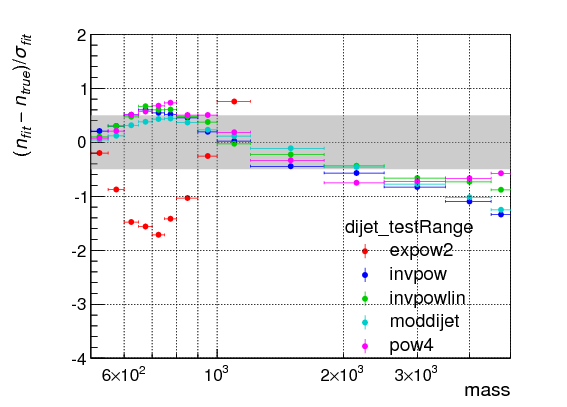
\includegraphics[width = .45\textwidth]{figures/diphotons/profile_pull_dijet_testRange_EBEB.png}
    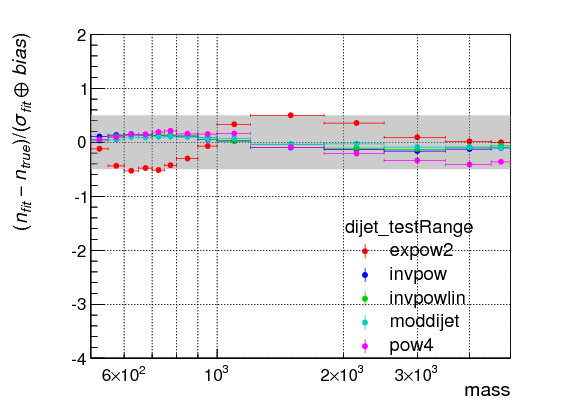
\includegraphics[width = .45\textwidth]{figures/diphotons/profile_corr_pull_dijet_testRange_EBEB.png}
    \caption{
      Median of the pull $p$ and modified pull $\tilde p$ for all considered test
      regions according to Tab.~\ref{tab:bias_regions} for EBEB. Different datasets correspond to different truth models as specified in the text.
      \label{fig:profile_bias_EBEB}
}
\end{figure}
\begin{figure}[!h]
    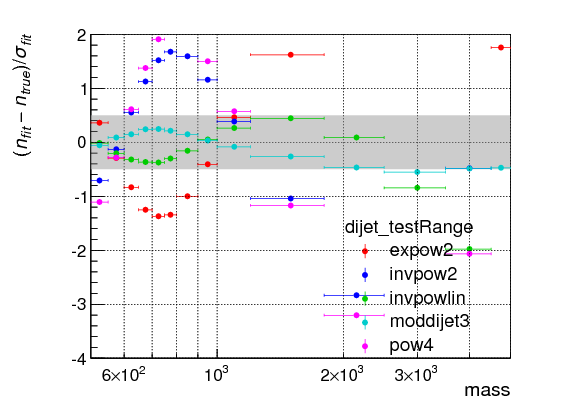
\includegraphics[width = .45\textwidth]{figures/diphotons/profile_pull_dijet_testRange_EBEE.png}
    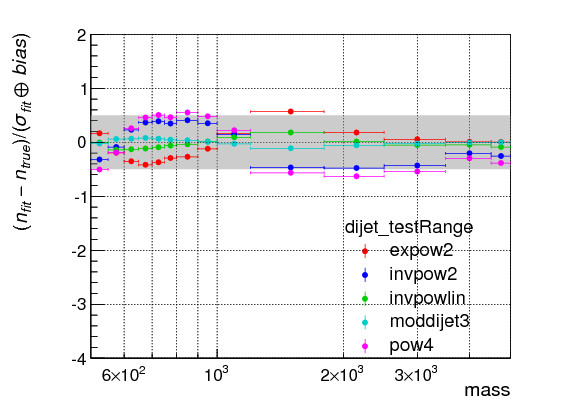
\includegraphics[width = .45\textwidth]{figures/diphotons/profile_corr_pull_dijet_testRange_EBEE.png}
    \caption{
      Median of the pull $p$ and modified pull $\tilde p$ for all considered test
      regions according to Tab.~\ref{tab:bias_regions} for EBEE. Different datasets correspond to different truth models as specified in the text.
      \label{fig:profile_bias_EBEE}
}
\end{figure}

The size of the background mismodeling enters the hypothesis test as the only
systematic uncertainty on the background model. The shape of this additional bias is
assumed to have a similar form as the signal PDF (S(\mgg)) and is therefore modeled
as a Gaussian of mean zero and with a width, that reflected the size of the bias. It is
added to the background description via the following equation in which $N_{bkg} (N_{\beta})$ are
the number of background (bias) events:

\begin{equation}
    \tilde{g}_{sig}(\mgg|\theta_{\beta}) \cdot Pdf(\theta_{\beta}) = \left ( \frac{
          N_{bkg} - \theta_{\beta} N_{\beta}(sig) } {N_{bkg}} g(\mgg) + \frac
    {\theta_{\beta} N_{\beta}(sig)} {N_{bkg}} s(\mgg) \right ) \cdot Norm(\theta)
\label{eq:bkgspurious}
\end{equation}

Where $N_{\beta}(sig) = \int \beta(\mgg) \cdot s(\mgg) \sim \beta(m_{G}) \cdot FWHM(sig)$,
$S(\mgg)$ is the signal PDF and $Norm(x)$ is the normal distribution.

%% SIGNAL
\clearpage
\subsection{Signal model}

In order to statistically interpret the data, it is necessary to have a description of both the signal shape
of the diphoton mass distribution and its normalization as a function of the predicted signal mass.
The signal shapes, which are mainly dominated by the detector and reconstruction response in the ECAL,
need to be well described in each of the two events categories.

\subsubsection{Signal shape parametrization}
\label{sec:signal_shape}
This section describes the technique used to describe the shape of the resonant diphoton signal with a parametric model. 
The use of a parametric description of the shape 
allows to perform a fine scan of the investigated mass without the need of generating an 
infinite number of signal simulation samples.

The Monte Carlo simulation signal samples are used to build a model for the signal.
The energy resolution smearing and efficiency scale factors 
described in Section~\ref{sec:dipho_energy} are applied.
The strategy is to describe the simulated signal with an analytic function in which the hypothetical signal mass ($m_{X}$)
represents a parameter which can vary continuously for any value in the range of interest of the search, while
the width of the resonance is fixed to the three benchmarks values chosen for this analysis.
The procedure is the following:

\begin{itemize}
\item The response distribution of the reduced mass ($\Delta m$) is computed for each mass point for which the
  full event simulation and reconstruction was performed.
  The reduced mass is computed as the difference between
  the reconstructed diphoton mass in the event ($m_{reco}$)
  and the true mass ($m_{true}$) of the event: $\Delta m = m_{reco}-m_{true}$

\item In order to construct the parametric model the response distribution is fitted with an analytic function, namely a double-sided  Crystal-Ball function  with  mean $m_0$,  sigma $\sigma$ and two asymmetric tails defined by two different different $n$ and $\alpha$ parameters. The Crystal-Ball function (CB) $f_{CB}(x)$  combines a Gaussian core and a power-law tail with an exponent $n$ to account for photon energy loss due to pair production.
%\begin{equation}
%f_{CB}(x) =  \begin{cases} \frac{N}{\sqrt{2\pi}\sigma}exp(-\frac{(x-x_0)^2}{2\sigma^2}), & \mbox{for  } \frac{x-x_0}{\sigma}>\alpha; \\ \frac{N}{\sqrt{2\pi}\sigma}\left ( \frac{n}{|\alpha|}\right )^n exp (-\frac{|\alpha|^2}{2}) \left ( \frac{n}{|\alpha|}- |\alpha|-\frac{x-x_0}{\sigma}\right )^{-n}   & \mbox{for  } \frac{x-x_0}{\sigma} \le \alpha  \end{cases}
%\label{cbfcn}
%\end{equation}
The parameter $\alpha$ defines the transition between the Gaussian and the power-law functions. 
In Figure~\ref{fig:fitRes1250} the fit to the reduced mass is shown for one of the signal mass point ($m_X = 1250$ GeV).

\item The theoretical signal line shape of the $X$ resonance is described by the functional form of a relativistic Breit-Wigner centered at $m_X$ and with the expected natural width for a resonance of $\Gamma_X$. The Breit-Wigner distribution is fitted in this analysis with a double-sided crystal-ball. The results of the fit are shown in Figure~\ref{fig:bw1250} for $m_X=1250$ GeV.

\item The theoretical line-shape fit function is convolved with the response fit function  to account for the experimental resolution of the ECAL. The convolved shape is compared with the reconstructed mass shape as a closure test of the fitting model. The closure test is shown in Figure~\ref{fig:reco1250} for $m_X=1250$ GeV.

\item The convolved model obtained in the previous step is used to throw an Asimov dataset which is fitted with a double-sided crystal-ball. This ultimate fitting model represents the final description of the mass resonance for a given mass and width. The closure test fit to the asimov dataset is shown in Figure~\ref{fig:final1250} for $m_X=1250$ GeV  narrow width.

\item The signal model derived in the previous steps depends continuously upon  $m_X$ through the parameters which describes the model itself: mean, $sigma$, $\alpha_{L/R}$, $n_{L/R}$. For each category and for each width hypothesis the trend of these parameters is studied and modelled with a polynomial function with $m_X$ as the only independent variable. Figures~\ref{fig:fitmean} show an example fit to one of the  double-sided crystal-ball parameters for the $\Gamma / \mgg = 1.4\%$ width hypothesis. The width of the Gaussian core is, among the model parameters, the one that affect the most the final results since
  a change in the width (i.e. better or worse resolution) directly impact the local signal over background ratio.

\end{itemize}
  
\begin{figure}[!h]
\begin{center}
  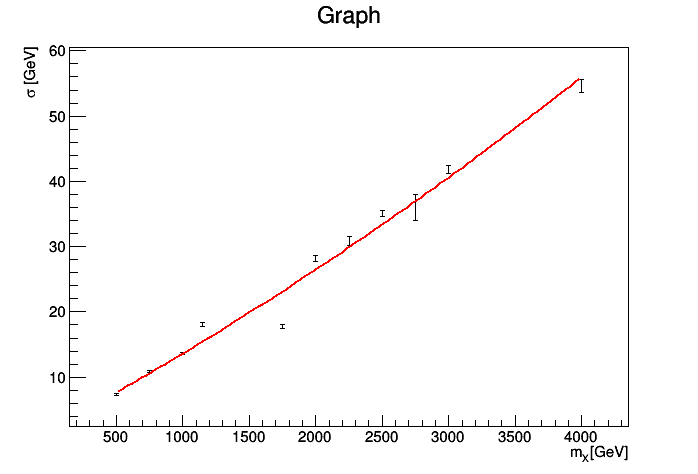
\includegraphics[width=0.7\textwidth]{figures/diphotons/sigmaVsMass_EBEB016.png}
  % 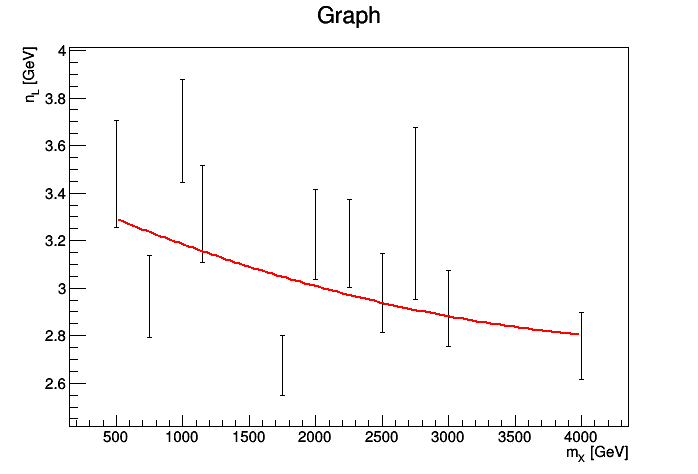
\includegraphics[width=0.45\textwidth]{figures/diphotons/nLVsMass_EBEB016.png}
  % 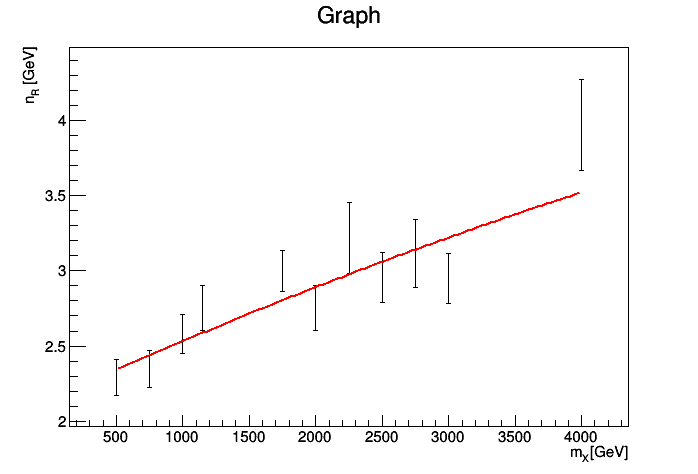
\includegraphics[width=0.45\textwidth]{figures/diphotons/nRVsMass_EBEB016.png}
  % 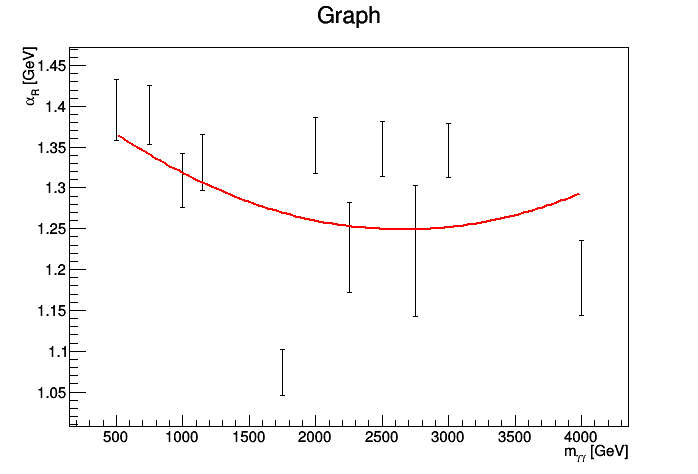
\includegraphics[width=0.45\textwidth]{figures/diphotons/aRVsMass_EBEB016.png}
  % 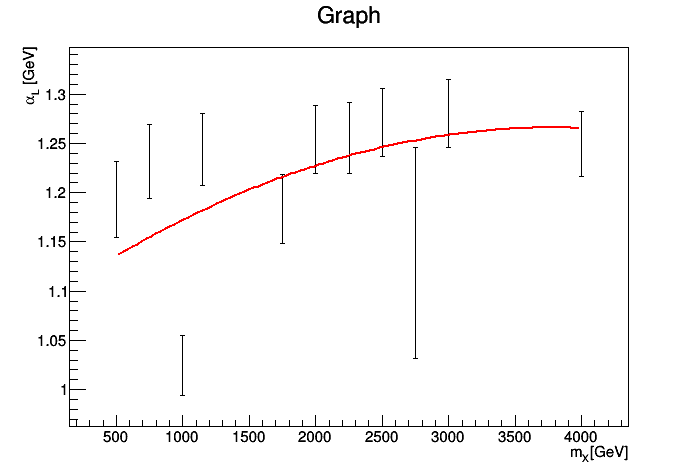
\includegraphics[width=0.45\textwidth]{figures/diphotons/aLVsMass_EBEB016.png}
 \caption{Double-sided crystal-ball $\sigma$ parameter modelling as a function of $m_X$. The Fit is performed with a polynomial function. Only fits to the EBEB category for medium width hypothesis are shown here.}
\label{fig:fitmean}
\end{center}
\end{figure}

\begin{figure}[!h]
 \begin{center}
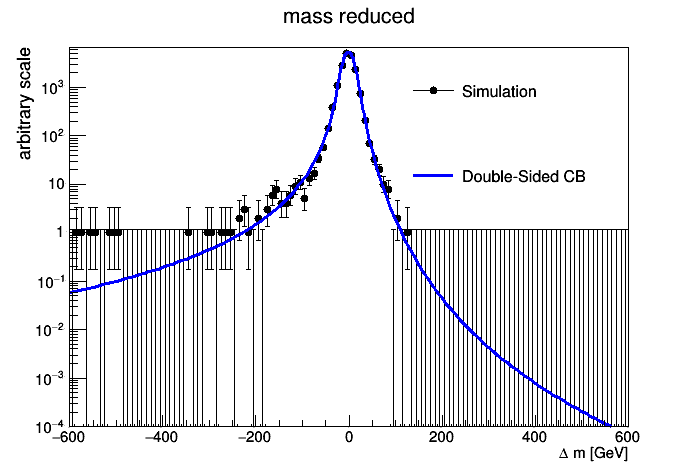
\includegraphics[width=0.45\textwidth]{figures/diphotons/responsefcnfitcbcb_EBEB016_M1250_k001_log.png}
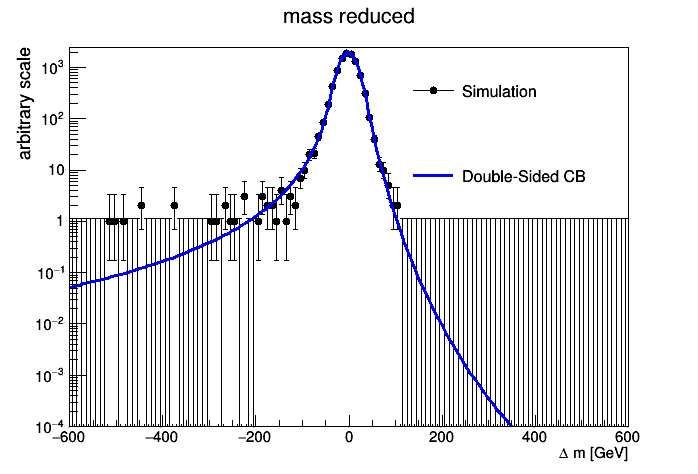
\includegraphics[width=0.45\textwidth]{figures/diphotons/responsefcnfitcbcb_EBEE016_M1250_k001_log.png}
  \caption{Double-sided Crystal-Ball fit (blue line) to the response distributions for $m_X=1250$ GeV. EBEB category on the left and EBEE category on the right}
 \label{fig:fitRes1250}
 \end{center}
\end{figure}
  
\begin{figure}[!h]
 \begin{center}

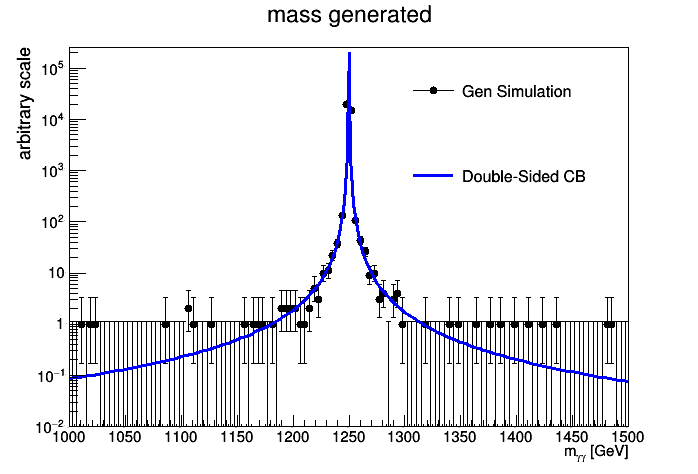
\includegraphics[width=0.45\textwidth]{figures/diphotons/mgen_cat4_M1250_k001_log.png}
\caption{Double-sided Crystal-Ball fit (blue line) to the generator-level distributions for $m_X=1250$ GeV narrow width hypothesis.}
 \label{fig:bw1250}
 \end{center}
\end{figure}

\begin{figure}[!h]
 \begin{center}
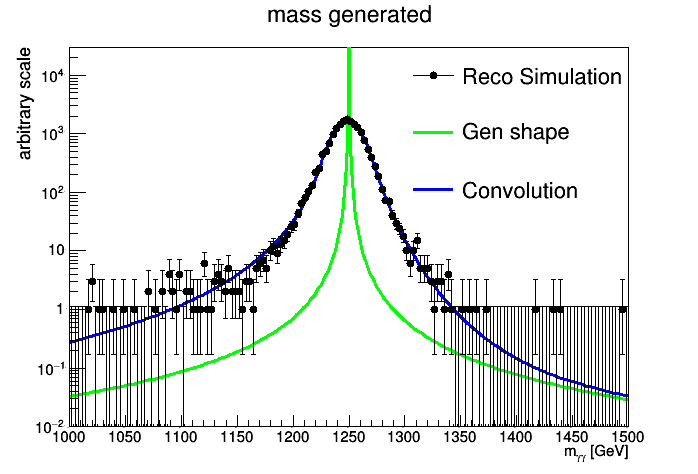
\includegraphics[width=0.45\textwidth]{figures/diphotons/mreco_EBEB016_M1250_k001_log.png}
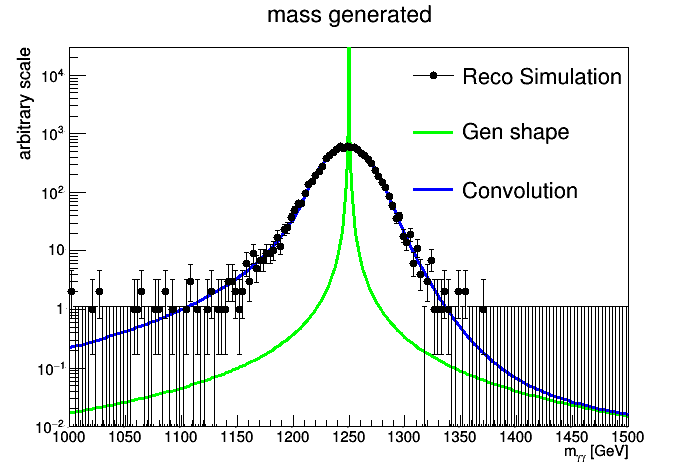
\includegraphics[width=0.45\textwidth]{figures/diphotons/mreco_EBEE016_M1250_k001_log.png}
  \caption{Convolved model (blue line) of the response function and the generator-level function (green line) compared to the reconstructed mass distribution for $m_X=1250$ GeV. EBEB category on the left and EBEE category on the right.}
 \label{fig:reco1250}
 \end{center}
\end{figure}
  
\begin{figure}[!h]
 \begin{center}
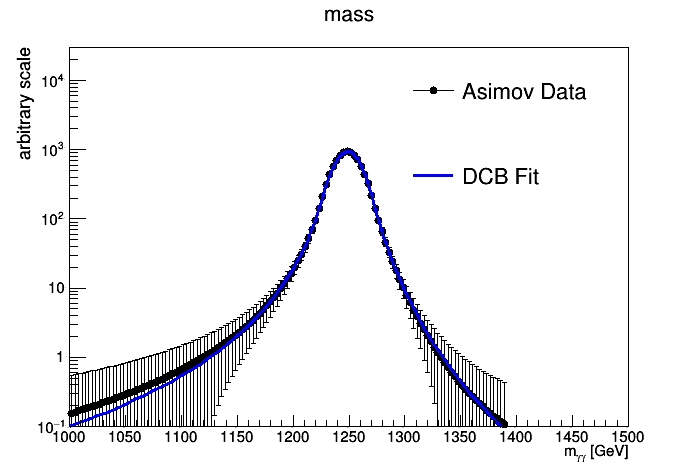
\includegraphics[width=0.45\textwidth]{figures/diphotons/fitasimov_EBEB016_M1250_k001_log.png}
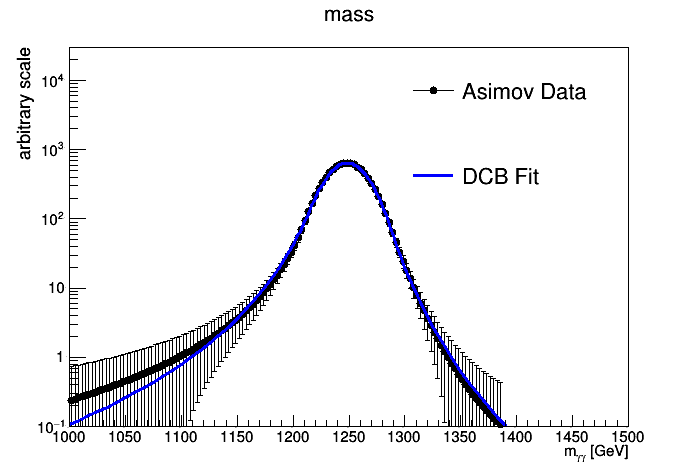
\includegraphics[width=0.45\textwidth]{figures/diphotons/fitasimov_EBEE016_M1250_k001_log.png}
  \caption{Convolved model (blue line) of the response function and the generator-level function (green line) compared to the reconstructed mass distribution  for $m_X=1250$ GeV. EBEB category on the left and EBEE category on the right.}
 \label{fig:final1250}
 \end{center}
\end{figure}

\subsubsection{Signal normalization}
In order to determine the signal normalization, the event selection efficiency
described in Section~\ref{sec:dipho_eff} is combined with the kinematic acceptance.
The total combined efficiency and acceptance ($\epsilon\times A$)
varies between 0.5 and 0.7 (0.6) for the spin-2 (spin-0) model and is shown in Figure~\ref{fig:eff_times_acc}. The EBEB
category has a higher sensitivity than the EBEE category and contributes to the overall
$\epsilon\times A$ with more than $50\%$ for lower $m_X$ values and up to $85\%$ for high $m_X$ values. Since
the diphoton selection efficiency stays flat over the \mgg spectrum (Figure~\ref{fig:eff_reco_sig}), any
visible trends are mainly driven by the signal acceptance.

\begin{figure}[h!]
  \centering
  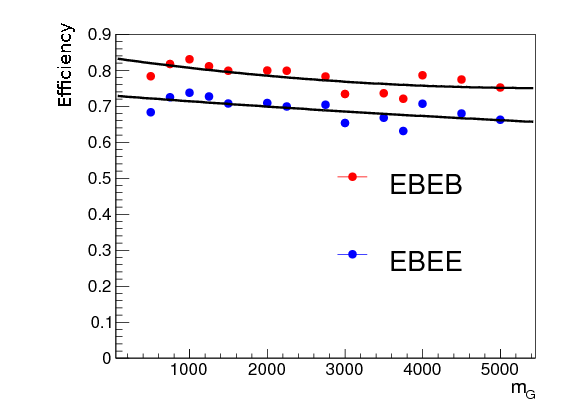
\includegraphics[width = 0.7\textwidth]{figures/diphotons/avg_eff_reco.png}
  \caption{diphoton identification selection efficiency as a function of the generated resonance mass.
    The efficiency used in the signal model normalization is parametrized with a second order polynomial (black curve)
    separately for the EBEB (red) and EBEE (blue) categories.}
  \label{fig:eff_reco_sig}
\end{figure}

The acceptance of the spin-0 signal model is mostly flat over the $m_X$ spectrum,
whereas for the spin-2 RS-Graviton signal it rises with larger $m_X$ values.
The angular distribution of the decay products of a spin-0 resonance is isotropic 
whereas that of those coming from a spin-2 one is not and one of the two photon is more likely
to be produced along the beam direction.
For this reason the geometric acceptance for a spin-0 signal is larger than that of a spin-2
almost at any $m_X$ value. Only a high masses (above 4 TeV) the spin-2 is larger than that of spin-0.
Spin-0 resonances can only be produced through gluon-fusion mechanism in p-p collisions while
spin-2 ones can also be produced through quark-antiquark annihilation; since
the gluon p.d.f decreases rapidly with the fraction of the proton momentum carried by the gluon while 
the quark p.d.f peaks at large momentum fraction values, for $m_X$ values larger than 4 TeV a significant
part of the spin-0 signal is produced off-shell and is rejected by kinematic selections while for spin-2
the effect is compensated by a larger production through quark-antiquark annihilation.

\begin{figure}[!h]
  \centering
  \includegraphics[width = .7\textwidth]{figures/diphotons/param_eff_acc.pdf}
  \caption{Fraction of events selected by the analysis categories for
    $0.5 < m_X < 4.5$ TeV and the narrow width hypothesis $\Gamma_X/m_X = 1.4\times 10^{-4}$.
    Curves for both spin-0 and RS-graviton resonances are shown.}
  \label{fig:eff_times_acc}
\end{figure}

\clearpage
\subsection{Source of systematic uncertainties}
\label{sec:syst}
Although the dominant uncertainty of the analysis is of statistical origin, various sources of systematic
uncertainty are considered.

All normalization uncertainties are assigned to the signal yield and are
reported in the following list:

\begin{itemize}
\item {\bf Luminosity uncertainty:} 2.5\% on the signal normalization was assigned to
    reflect the uncertainty on the knowledge of the total integrated luminosity.
\item {\bf Selection efficiency uncertainties:} a 6\% uncertainty on the signal
    normalization was included to reflect the uncertainty on the knowledge of the
    data/simulation scale factors. This value is equivalent to two times the total uncertainty of the last $p_T$ bin of
    Figure~\ref{fig:tnp}. Although the chosen value is very conservative the effect on the final results is very
    small given their relative larger statistical uncertainty.
\item {\bf Parton distribution functions: } a 6\% uncertainty on the signal normalization
    was assigned in order to account for the variation in the kinematic acceptance of the
    analysis coming from the use of alternative PDF sets.
\item {\bf Photon energy scale uncertainty:} a 1\% energy scale uncertainty was assumed. 
    This number was derived to take into account the knowledge of the energy scale uncertainty at the Z peak as well 
    as the knowledge on the extrapolation to high mass.
\item {\bf Photon resolution uncertainty} The uncertainty on the extra smearing on the
    photon uncertainty was evaluated summing and subtracting be 0.5\% in quadrature from
    the estimated constant term measured at the Z peak. The 0.5\% value was chosen to
    match the statistical uncertainty on the extra smearing term measured with the
    non-resonant Drell-Yan production.
\end{itemize}

The parametric background model has no associated systematic uncertainties, except for the
bias term uncertainty described in Section~\ref{sec:background}.
The shape coefficients are treated as unconstrained nuisance parameters and contribute to
the statistical uncertainties.

\clearpage
\section{Results on the search for BSM resonant diphoton production}
The standard LHC test statistic $q(\mu)$ is used to provide a statistical interpretation of the results:

\begin{equation}
 q(\mu) = -log \lambda(\mu) := -log \frac{ L(\mu \cdot S + B | \underline{\hat\theta}_{\mu} ) } {L (\hat\mu
  \cdot S + B | \underline{\hat\theta} )}
\end{equation}
\label{eq:test_stat}

Where the likelihood is the one described in Section~\ref{sec:results},
$S$ and $B$ are the pdf's for the signal and SM processes respectively, $\mu$ is
the ``signal strength'' parameter and $\underline\theta$ are the nuisance parameters of
the model. The $\hat{}$ notation indicate best-fit value of the parameters.

The value of $\lambda$ is bounded between 0 and 1, where the latter denotes a good agreement between the
observed data and the hypothesized value of $\mu$. Consequently, the higher the value of
the test statistic $q(\mu)$, the higher the incompatibility between the observed data and the
hypothesized signal model with signal strength $\mu$.
The discovery of a new diphoton resonance would appear as a localized excess of events.
The SM background only hypothesis is the null hypothesis in the test and correspond to $\mu = 0$.

Since no significant deviation from the SM prediction is observed in data in the search region ($\mgg > 500$ GeV)
Upper exclusion limits on the resonant diphoton production rate under different signal
hypotheses are set using the modified frequentist method, which is a standard method among searches
for BSM physics at LHC. It is also known
as the $CL_s$ method [164, 165]. The signal plus background hypothesis ($H_1$) 
is tested against the alternative, background-only hypothesis ($H_0$). For
upper limits, the test statistic $q(\mu)$ of Equation~\ref{eq:test_stat} is defined as [163]:

\begin{equation}
  \tilde{q}(\mu) = \begin{cases}
    -2~ln(\lambda(\mu)), & 0 \leq \hat\mu \leq \mu. \\
    0 & \hat\mu > \mu.
  \end{cases}
\end{equation}  

the lower bound $\hat\mu \geq 0$ is  dictated  by  physics  (signal  rate  is  positive),  while
the upper constraint $\hat\mu \leq \mu$ is imposed by hand in order to guarantee a one-sided
confidence interval which in turn ensures that upward fluctuations in data are not considered as
evidence against the signal plus background hypothesis.

Two probabilities are defined, one for the signal plus background hypothesis
($CL_{s+b} = P( \tilde{q}_{\mu} \geq \tilde{q}_{\mu,obs} |H_1 )$) and
one for the background-only hypothesis ($CL_b = P( \tilde{q}_{\mu} \geq \tilde{q}_{\mu,obs} |H_0 )$). The $CL_s$ is defined
as the ratio of the two probabilities and depends on the tested signal strength $\mu$:
\[
  CL_s = \frac{CL_{s+b}}{CL_b}
\]

The $CL_s$ value needs to be smaller than a threshold $\alpha$ to exclude the tested signal model ($H_1$ hypothesis) 
with signal strength $\mu$ at a confidence level ($CL$) of $(1-\alpha)$. This chosen threshold is 0.05,
corresponding to a $95\%$ $CL_s$ limit. The above probabilities $CL_b$ and $CL{s+b}$
are calculated for different values of $\mu$. All possible $q_{\mu}$ are tested until a signal strength
that gives a $CL_s$ value lower than $\alpha = 0.05$ is found.

Throughout the calculations the asymptotic formulas described in~\cite{Cowan:2010js} are used.

\clearpage
\subsection{Exclusion limits on the production of spin-0 and spin-1 resonances}
As previously stated two models are considered as benchmarks in this search for resonances decaying to two photos:
\begin{itemize}
\item \RS gravitons (spin-2).
\item spin-0 resonances produced via gluon-fusion.
\end{itemize}

For each of the hypotheses, three different width $\Gamma / M$ are considered:
0.014\%, 1.4\% and 5.6\%. In the case of the RS graviton resonances, the width is
parametrized as $\Gamma / M = 1.4 k^2$ and thus k=0.01,0.1,0.2. The three values are representative of
three different scenario: the narrowest reflect the case of an intrinsic width negligible with respect to the
detector resolution (i.e. the ECAL energy resolution), the second reflect the case of a resonance width
comparable to the detector resolution and the third the case of a resonance with a intrinsic width larger than
the mass resolution.

The median expected and observed exclusion limits for different signal hypotheses are shown in
Figure~\ref{fig:limits} for \RS graviton and gluon-fusion-produced spin-0 resonances of different widths.

\begin{figure}[h!]
  \centering
  \includegraphics[width = 0.45\textwidth]{figures/diphotons/spin2/limits_k001.pdf}
  \includegraphics[width = 0.45\textwidth]{figures/diphotons/spin0/limits_k001.pdf}\\
  \includegraphics[width = 0.45\textwidth]{figures/diphotons/spin2/limits_k01.pdf}
  \includegraphics[width = 0.45\textwidth]{figures/diphotons/spin0/limits_k01.pdf}\\
  \includegraphics[width = 0.45\textwidth]{figures/diphotons/spin2/limits_k02.pdf}
  \includegraphics[width = 0.45\textwidth]{figures/diphotons/spin0/limits_k02.pdf}\\
    \caption{
      Expected and observed upper limit for \RS graviton (left) and gluon-fusion-produced spin-0
      (right) resonances of different widths decaying to two photons:
      narrower (top) to wider (bottom). For \RS graviton the expected cross-section times branching fraction
      for the decay to two photons is shown by the dashed red curve. The limits are shown as a function of
      the reconstructed diphoton invariant mass.
    }
    \label{fig:limits}
\end{figure}

\subsection{Exclusion limits on the fiducial cross-section for resonant diphoton production}
The same set of events can be interpreted setting a limit on the resonant diphoton production cross-section.
This approach allows one to compare the experimental results with the prediction from any model; the
only assumption are dictated by the width of the resonance and the shape of the signal, which is assumed to
be the same double-sided crystal ball function described in Section~\ref{sec:signal_shape}.

The limits are set independently for the EBEB and EBEE categories and the
fiducial volume is defined by a set of selections applied to the simulated signal sample on generator
level quantities reported below:
\begin{itemize}
\item The generator level transverse momentum of each of the two photons grater than 75 GeV.
\item Generetor level isolation ($Iso_{\gamma}^{gen}$) less than 10 GeV. Where $Iso_{\gamma}^{gen}$ is defined as:
  \[
    Iso_{\gamma}^{gen} = \sum p_T
  \]
  The sum runs over all the generator level particles, regardless of the type, included within a cone of radius $\Delta R = 0.3$
  around the direction of the photon in the $\eta$-$\phi$ plane.
\item Detector acceptance: $|\eta_{\gamma 1,2}^{gen}| < 1.442$ for the EBEB category and
  $|\eta_{\gamma 1}^{gen}| < 1.442$, $1.556 < |\eta_{\gamma 2}^{gen}| < 2.5$ for the EBEE one.
\end{itemize}

The signal normalization is determined by the selection efficiency reported in Figure~\ref{fig:eff_reco_sig}.
The background estimation and systematic uncertainties on the signal yield are the same as for the benchmark model
results (Section~\ref{sec:syst}) except for the uncertainty introduced by the variation of the parton density functions, which
is irrelevant in this case.

The median expected and observed exclusion limits for the model independent diphoton resonant production 
are shown in Figure~\ref{fig:limits} for the two event categories and the three relative width considered in the analysis

\begin{figure}[h!]
  \centering
  \includegraphics[width = 0.45\textwidth]{figures/diphotons/fid_EBEB/limits_k001.pdf}
  \includegraphics[width = 0.45\textwidth]{figures/diphotons/fid_EBEE/limits_k001.pdf}\\
  \includegraphics[width = 0.45\textwidth]{figures/diphotons/fid_EBEB/limits_k01.pdf}
  \includegraphics[width = 0.45\textwidth]{figures/diphotons/fid_EBEE/limits_k01.pdf}\\
  \includegraphics[width = 0.45\textwidth]{figures/diphotons/fid_EBEB/limits_k02.pdf}
  \includegraphics[width = 0.45\textwidth]{figures/diphotons/fid_EBEE/limits_k02.pdf}\\
    \caption{
      Expected and observed upper limit for the EBEB (left) and EBEE (right) categories for a generic
      resonant production of diphoton pairs as a function of the reconstructed diphoton invariant mass.
      Three different relative resonance width hypothesis are considered: $\Gamma/m = 0.014\%$(top), $1.4\%$(middle) and $5.6\%$(bottom).
    }
    \label{fig:fiducial_limits}
\end{figure}

\section{Summary}
\label{sec:dipho_summary}
The search for local excesses in the diphoton spectrum compatible with the prediction of wrapped extra dimension models
for the production of a massive spin-2 boson and spin-0 Higgs-like boson predicted by MSSM models
has been performed using data collected by the CMS experiment during 2016.

The observed data are compatible with the standard model prediction through all the analyzed part of the diphoton
spectrum. In particular the results exclude the existence of a RS-graviton with masses below $2.1$ TeV and $\kappa = 0.01$.
The excluded region extends more than $\sim 4$ TeV for wider resonances with $\kappa =$ 0.1 and 0.2.
The results are compatible with those presented by a similar search performed by the ATLAS collaboration with
data collected during the same period~\cite{atlas_dipho_2016}.
These results extend the sensitivity of those previously published by CMS with data collected at both 8 and 13 TeV
LHC center of mass energies~\cite{cms_dipho_2015, cms_dipho_2012_1, cms_dipho_2012_2}.

No combination of the results with those collected at 8 TeV is done since with an integrated luminosity of \lumisix
the sensitivity of the analysis performed with data at 13 TeV dominates over the 8 TeV one.